%%%%%%%%%%%%%%%%%%%%%%%%%%%%%%%%%%%%%%%%%
% Arsclassica Article
% LaTeX Template
% Version 1.1 (10/6/14)
%
% This template has been downloaded from:
% http://www.LaTeXTemplates.com
%
% Original author:
% Lorenzo Pantieri (http://www.lorenzopantieri.net) with extensive modifications by:
% Vel (vel@latextemplates.com)
%
% License:
% CC BY-NC-SA 3.0 (http://creativecommons.org/licenses/by-nc-sa/3.0/)
%
%%%%%%%%%%%%%%%%%%%%%%%%%%%%%%%%%%%%%%%%%

%----------------------------------------------------------------------------------------
%	PACKAGES AND OTHER DOCUMENT CONFIGURATIONS
%----------------------------------------------------------------------------------------

\documentclass[
12pt, % Main document font size
a4paper, % Paper type, use 'letterpaper' for US Letter paper
oneside, % One page layout (no page indentation)
%twoside, % Two page layout (page indentation for binding and different headers)
headinclude,footinclude, % Extra spacing for the header and footer
BCOR5mm, % Binding correction
]{scrartcl}
%%%%%%%%%%%%%%%%%%%%%%%%%%%%%%%%%%%%%%%%%
% Arsclassica Article
% Structure Specification File
%
% This file has been downloaded from:
% http://www.LaTeXTemplates.com
%
% Original author:
% Lorenzo Pantieri (http://www.lorenzopantieri.net) with extensive modifications by:
% Vel (vel@latextemplates.com)
%
% License:
% CC BY-NC-SA 3.0 (http://creativecommons.org/licenses/by-nc-sa/3.0/)
%
%%%%%%%%%%%%%%%%%%%%%%%%%%%%%%%%%%%%%%%%%

%----------------------------------------------------------------------------------------
%	REQUIRED PACKAGES
%----------------------------------------------------------------------------------------

\usepackage[
nochapters, % Turn off chapters since this is an article        
beramono, % Use the Bera Mono font for monospaced text (\texttt)
eulermath,% Use the Euler font for mathematics
pdfspacing, % Makes use of pdftex’ letter spacing capabilities via the microtype package
dottedtoc % Dotted lines leading to the page numbers in the table of contents
]{classicthesis} % The layout is based on the Classic Thesis style

\usepackage{arsclassica} % Modifies the Classic Thesis package

\usepackage[T1]{fontenc} % Use 8-bit encoding that has 256 glyphs

\usepackage[utf8]{inputenc} % Required for including letters with accents

\usepackage{graphicx} % Required for including images
\graphicspath{{Figures/}} % Set the default folder for images

\usepackage{enumitem} % Required for manipulating the whitespace between and within lists

\usepackage{lipsum} % Used for inserting dummy 'Lorem ipsum' text into the template

\usepackage{subfig} % Required for creating figures with multiple parts (subfigures)

\usepackage{amsmath,amssymb,amsthm} % For including math equations, theorems, symbols, etc

\usepackage{varioref} % More descriptive referencing

%----------------------------------------------------------------------------------------
%	THEOREM STYLES
%---------------------------------------------------------------------------------------

\theoremstyle{definition} % Define theorem styles here based on the definition style (used for definitions and examples)
\newtheorem{definition}{Definition}

\theoremstyle{plain} % Define theorem styles here based on the plain style (used for theorems, lemmas, propositions)
\newtheorem{theorem}{Theorem}

\theoremstyle{remark} % Define theorem styles here based on the remark style (used for remarks and notes)

%----------------------------------------------------------------------------------------
%	HYPERLINKS
%---------------------------------------------------------------------------------------

\hypersetup{
%draft, % Uncomment to remove all links (useful for printing in black and white)
colorlinks=true, breaklinks=true, bookmarks=true,bookmarksnumbered,
urlcolor=webbrown, citecolor=webgreen, % Link colors
pdftitle={}, % PDF title
pdfauthor={\textcopyright}, % PDF Author
pdfsubject={}, % PDF Subject
pdfkeywords={}, % PDF Keywords
pdfcreator={pdfLaTeX}, % PDF Creator
pdfproducer={LaTeX with hyperref and ClassicThesis} % PDF producer
} % Include the structure.tex file which specified the document structure and layout
\usepackage{fancybox}
%\usepackage{listings}
\usepackage{tikz}
\usepackage{xcolor}
%\usepackage{authblk}
%\usepackage{titlepic}
\usepackage{titling}


\hyphenation{Fortran hyphenation} % Specify custom hyphenation points in words with dashes where you would like hyphenation to occur, or alternatively, don't put any dashes in a word to stop hyphenation altogether


%----------------------------------------------------------------------------------------
%	TITLE AND AUTHOR(S)
%----------------------------------------------------------------------------------------

\title{\includegraphics[width=14cm,height=7cm]{Pictures/cado_logo_text_wide.png} \\ \normalfont\spacedallcaps{Installation Guide} \\
\vspace*{\fill}}% The article title

%\author[1]{Joshi, Saumitra}
%\author[1]{Medina, Juan Carlos}
%\author[1]{Menhorn, Friedrich}
%\author[1]{Reiz, Severin}
%\author[2]{R{\"u}th, Benjamin}
%\author[2]{Wannerberg, Erik}
%\author[2]{Yurova, Anna}
%\vfill{2cm}

%\author{Joshi, Saumitra; Medina, Juan Carlos; \\ Menhorn, Friedrich; Reiz, Severin;\\ R{\"u}th, Benjamin;  Wannerberg, Erik; Yurova, Anna}% The article author(s) - author affiliations need to be specified in the AUTHOR AFFILIATIONS block
%\author{
%\spacedlowsmallcaps{Saumitra Joshi, Juan Carlos Medina,} \\
%\spacedlowsmallcaps{Friedrich Menhorn, Severin Reiz,} \\
%\spacedlowsmallcaps{Benjamin R{\"u}th, Erik Wannerberg,} \\
%\spacedlowsmallcaps{Anna Yurova}
%}
%\author{
%{Saumitra Joshi, Juan Carlos Medina,} \\
%{Friedrich Menhorn, Severin Reiz,} \\
%{Benjamin R{\"u}th, Erik Wannerberg,} \\
%{Anna Yurova}
%}
%----------------------------------------------------------------------------------------

\begin{document}

%----------------------------------------------------------------------------------------
%	HEADERS
%----------------------------------------------------------------------------------------
\newcommand{\titlebox}[2]{
\begin{tikzpicture}
\node[draw,thick,inner sep=6mm] (titlebox) {#2};
\node[fill=white] (Title) at (titlebox.north) {\bfseries \large #1};
\end{tikzpicture}
}
\renewcommand{\sectionmark}[1]{\markright{\spacedlowsmallcaps{#1}}} % The header for all pages (oneside) or for even pages (twoside)

%\lehead{\mbox{\llap{\small\thepage\kern1em\{halfgray} \vline}\color{halfgray}\hspace{0.5em}\rightmark\hfil} % The header style
\newcommand{\titledframe}[2]{%
       \boxput*(0,1){\psframebox*{#1}}%
         {\psframebox[framesep=12pt]{#2}}}
         
\pagestyle{scrheadings} % Enable the headers specified in this block


%----------------------------------------------------------------------------------------
%	TABLE OF  CONTENTS & LISTS OF FIGURES AND TABLES
%----------------------------------------------------------------------------------------
\date{}
\maketitle % Print the title/author/date block
\thispagestyle{empty}

\setcounter{tocdepth}{2} % Set the depth of the table of contents to show sections and subsections only
\newpage
\setcounter{page}{1}
\tableofcontents % Print the table of contents



%----------------------------------------------------------------------------------------
%	ABSTRACT
%----------------------------------------------------------------------------------------

\section*{About} % This section will not appear in the table of contents due to the star (\section*)
This document provides general information about using the CADO software. CADO is a fully CAD-integrated topology optimization tool under the open source BSD license. It resulted from a project as part of the Bavarian Graduate School of Engineering at TU München and was developed by Saumitra Joshi, Juan Carlos Medina, Friedrich Menhorn, Severin Reiz, Benjamin R{\"u}th, Erik Wannerberg and Anna Yurova in 2015-2016.
%\begin{itemize}
%\item Saumitra Joshi
%\item Juan Carlos Medina
%\item Friedrich Menhorn
%\item Severin Reiz
%\item Benjamin R{\"u}th
%\item Erik Wannerberg
%\item Anna Yurova
%\end{itemize}

%----------------------------------------------------------------------------------------

\newpage % Start the article content on the second page, remove this if you have a longer abstract that goes onto the second page

%----------------------------------------------------------------------------------------
%	INTRODUCTION
%----------------------------------------------------------------------------------------

\section{ToPy}
\label{Topy}
	In our tool we use ToPy (\href{https://github.com/williamhunter/topy}{https://github.com/williamhunter/topy}) for topology optimization. 
\subsection{Prerequisites}
\label{ToPy:sec1}
	In order to install ToPy, make sure that the following software is installed on your computer:
\begin{itemize}
	\item Python (version 2.7)
	\item NumPy (Usually provided by Python distribution)
	\item PyVTK tool (\href{https://pypi.python.org/pypi/PyVTK}{https://pypi.python.org/pypi/PyVTK}) 
	\item Pysparse library (\href{http://pysparse.sourceforge.net/}{http://pysparse.sourceforge.net/})
\end{itemize}
	Here are some recommendations for the installation of the tools/libraries mentioned above.
	
	To install PyVTK tool, please run the following commands in your terminal:
\begin{itemize}
\item[] \texttt{\textbf{$>$ }sudo apt-get install python-pip}
\item[] \texttt{\textbf{$>$ }pip install pyvtk}
\end{itemize}
	
	The installation of the Pysparse library is a bit more cumbersome, since the pip-installation (like in the previous case) fails most of the times. So, here we provide an alternative way of installing Pysparse from the \textit{.git} repository.
	
	To install Pysparse (assuming the pip installation fails), make sure that \textit{git} (\href{https://git-scm.com/}{https://git-scm.com/}) is installed on your computer and then run the following commands in your terminal:
\begin{itemize}
\item[] \texttt{\textbf{$>$ }git clone git://pysparse.git.sourceforge.net/gitroot/ \\ pysparse/pysparse/}
\item[] \texttt{\textbf{$>$ }cd pysparse}
\item[] \texttt{\textbf{$>$ }sudo python setup.py install}
\end{itemize}
%	
\subsection{Install ToPy}
	If all the tools specified in the section \ref{ToPy:sec1} are installed, we can now proceed to the installation of ToPy itself. For that download ToPy from \href{https://github.com/williamhunter/topy}{https://github.com/williamhunter/topy}. 

For CADO it is necessary to have an output in the \textit{ascii} format. By default the output \textit{.vtk} files from ToPy are binary, so we need to change them to \textit{ascii}. In order to do that, please perform the following actions:
\begin{itemize}
 		\item Open the ToPy source file \textit{core/visualization.py}
 		\item Go to the method \texttt{{\_}write{\_}legacy{\_}vtu(x, fname)} in line 160

 		\item Change \textcolor{orange}{\texttt{'binary'}} to \textcolor{orange}{\texttt{'ascii'}} in line 194 (see pic. \ref{fig:ToPy_CodeChange})
\end{itemize} 
	
\begin{figure}
\centering
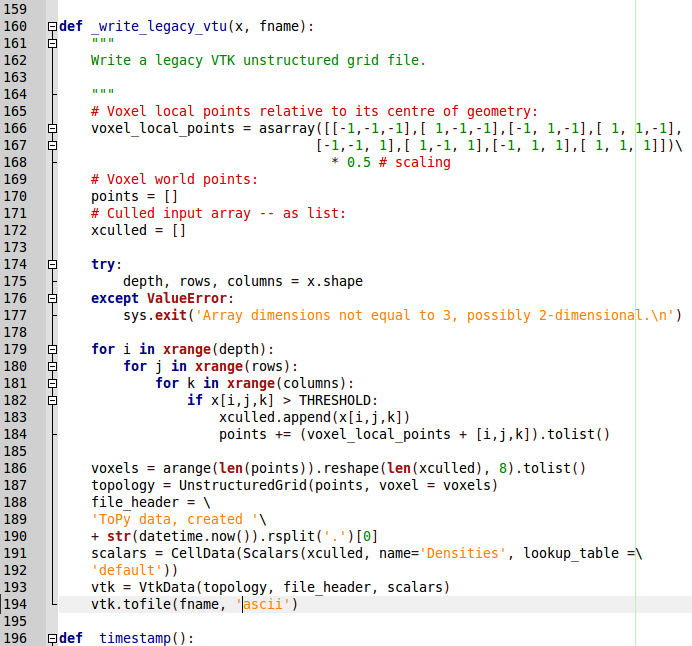
\includegraphics[scale=0.5]{img/ToPy_CodeChange.png}
\caption{Changing of the output type of ToPy to ascii}
\label{fig:ToPy_CodeChange}
\end{figure}

After making the following edit, run the following command from the root directory of ToPy:
\begin{itemize}
\item[] \texttt{\textbf{$>$ }sudo python setup.py install}
\end{itemize}

\begin{figure}
\centering
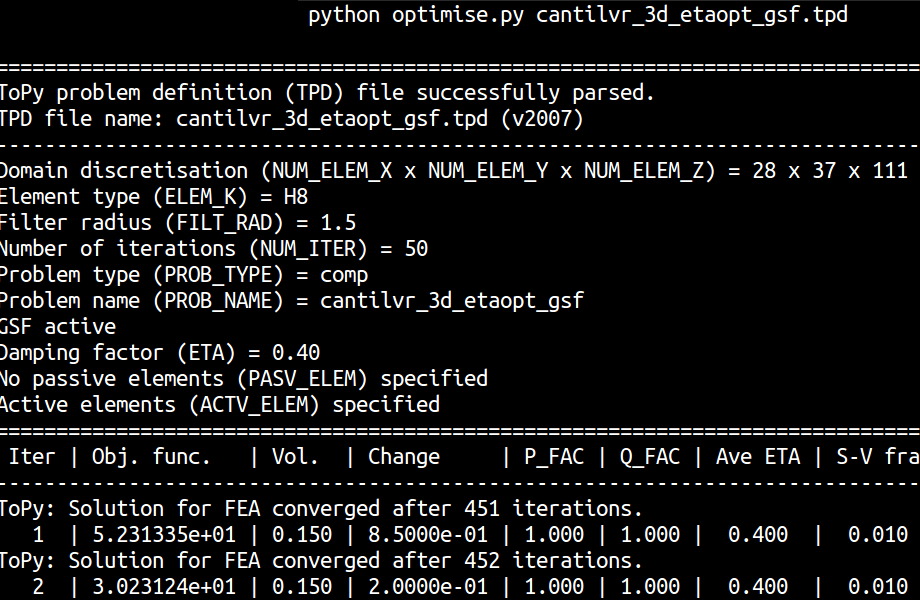
\includegraphics[scale=0.3]{img/ToPy_ExampleRun_cut.png}
\caption{ToPy test}
\label{fig:ToPy_test}
\end{figure}

\subsection{Test ToPy}
	In order to test whether the installation of ToPy was completed successfully it is possible to run some test cases provided in \textit{examples} folder. For that, do the following:
\begin{itemize}
	\item Enter one of the folders in examples \\(e.g. examples/cantilever)
	\item Execute a ToPy test run by running the following command in your terminal:
\begin{itemize}
	\item[] \texttt{\textbf{$>$ }python optimize.py $<$example.tpd-file$>$}
\end{itemize}
\end{itemize}
%
%\end{lstlisting}	
The output should look as showed in picture \ref{fig:ToPy_test}.

\section{OpenCascade}
\label{OpenCascade}
OpenCascade (\href{http://www.opencascade.com/}{http://www.opencascade.com/}) is an open-source CAD kernel. It is widely used in engineering and design for geometry construction and editing.
\subsection{Install OpenCascade}
For technical reasons, we do not use OpenCascade from the official webpage, but from the \textit{.git} repository. 
\begin{figure}
\centering
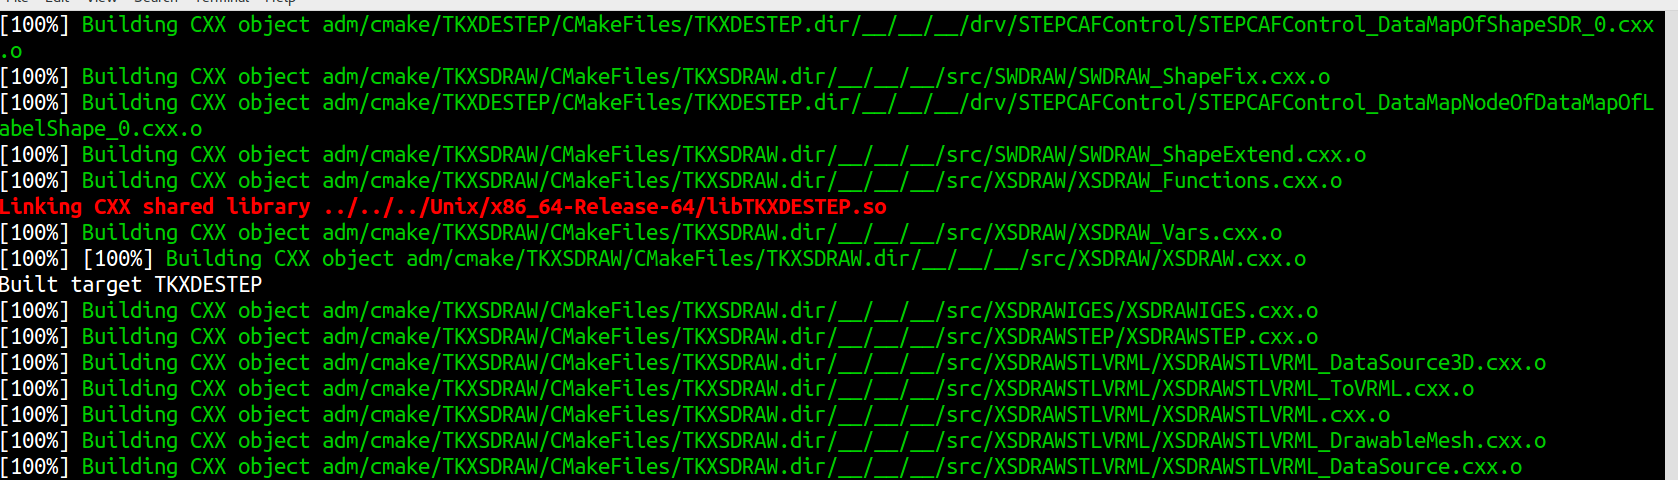
\includegraphics[scale=0.3]{img/OC_Build5_cut.png}
\caption{Building OpenCascade}
\label{fig:OC_build}
\end{figure}
\begin{figure}
\centering
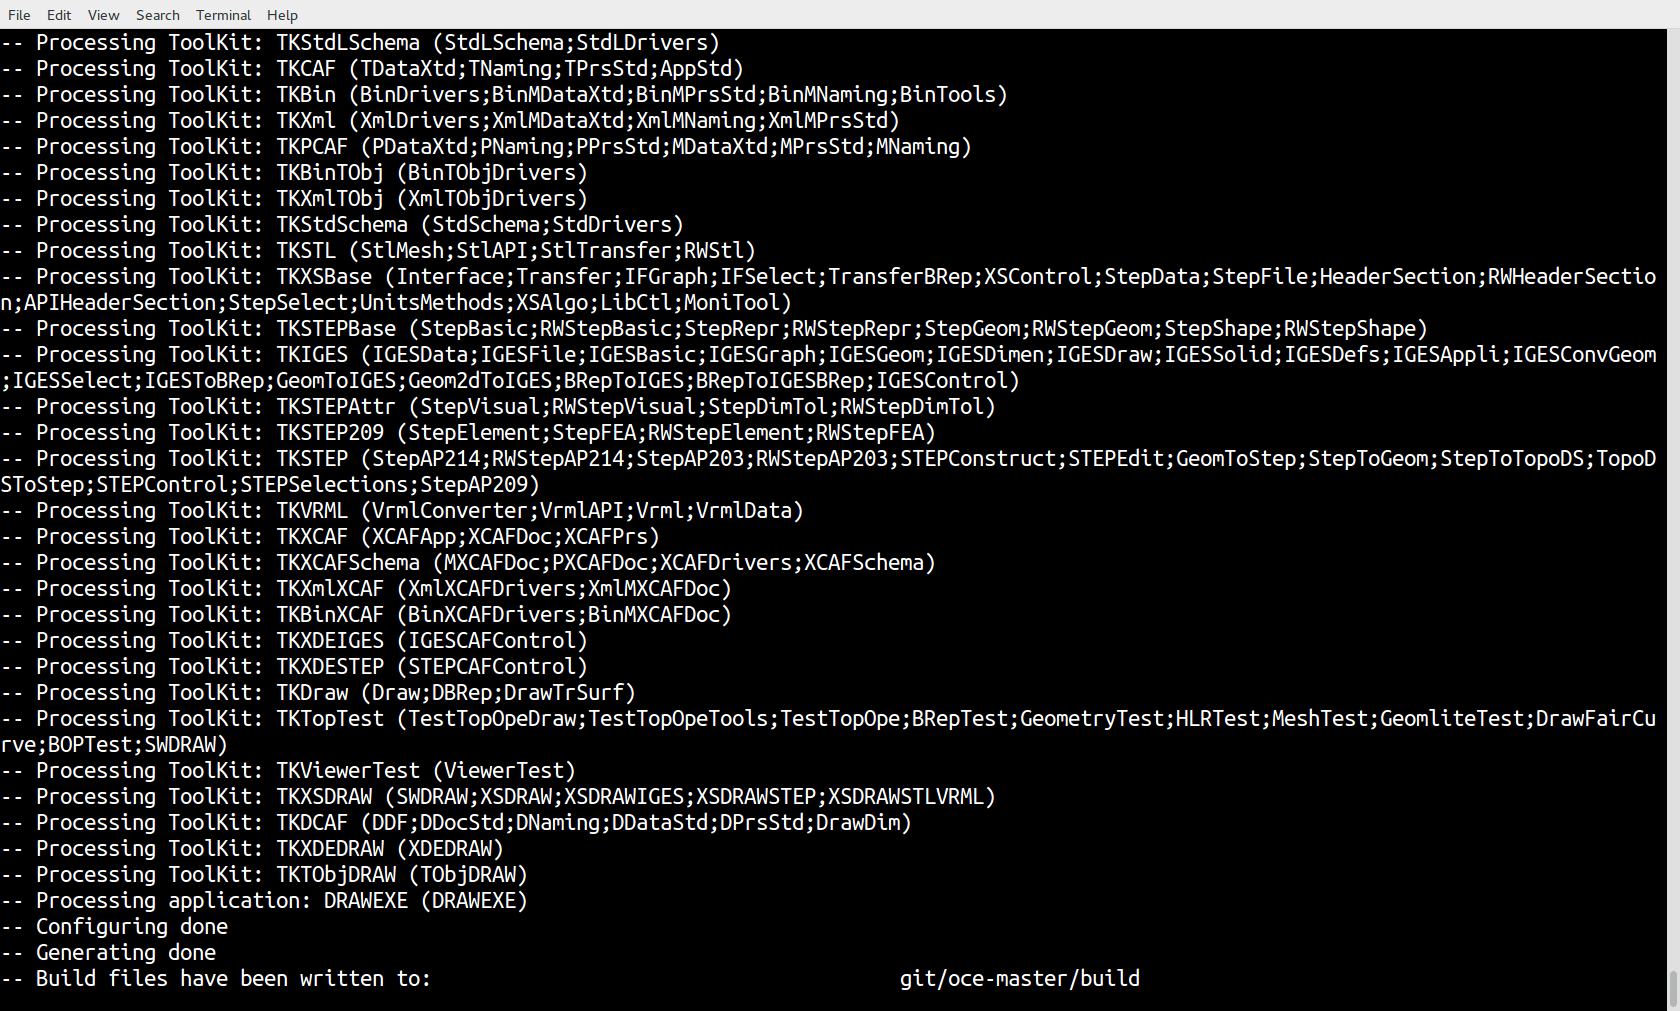
\includegraphics[scale=0.3]{img/OC_CMake2.png}
\caption{OpenCascade installation: cmake}
\label{fig:OC_cmake}
\end{figure}
To install OpenCascade this way, make sure that git (\href{https://git-scm.com/}{https://git-scm.com/}) is installed on your computer and then run the following commands in your terminal:
\begin{itemize}
\item Clone the repository:
\begin{itemize}
\item[] \texttt{\textbf{$>$ }git clone git://github.com/tpaviot/oce.git}
\item[] \texttt{\textbf{$>$ }cd oce}
\item[] \texttt{\textbf{$>$ }mkdir build}
\item[] \texttt{\textbf{$>$ }cd build}
\end{itemize}
\item Execute \texttt{cmake}:
\begin{itemize}
\item[] \texttt{\textbf{$>$ }cmake ..}
\end{itemize}
Sample output: see Pic. \ref{fig:OC_cmake}
\item Build OpenCascade:
\begin{itemize}
\item[] \texttt{\textbf{$>$ }make ..}
\end{itemize}
To speed up the process, build can be done in parrallel:
\begin{itemize}
\item[] \texttt{\textbf{$>$ }make -j<number\_of\_processors>}
\end{itemize}
Sample output: see Pic. \ref{fig:OC_build}
\item Install OpenCascade:
\begin{itemize}
\item[] \texttt{\textbf{$>$ }sudo make install ..}
\end{itemize}
Sample output: see Pic. \ref{fig:OC_install}
\end{itemize}

\begin{figure}
\centering
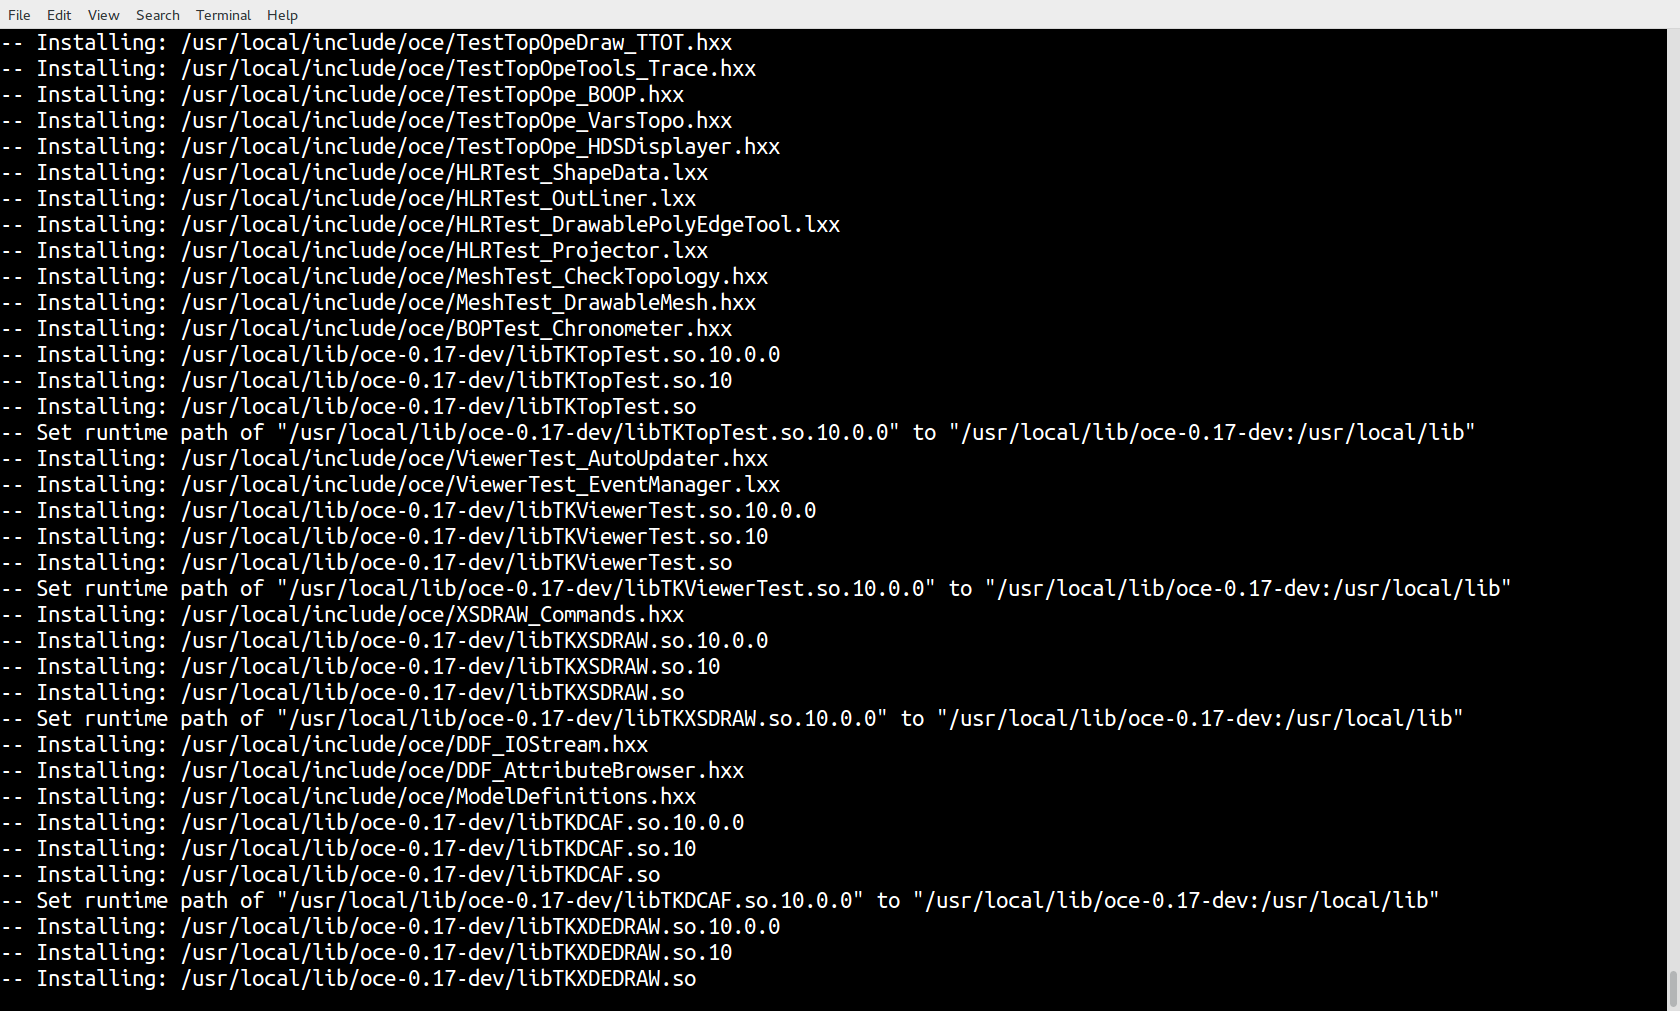
\includegraphics[scale=0.3]{img/OC_Install2.png}
\caption{OpenCascade installation}
\label{fig:OC_install}
\end{figure}
	 These steps are in accord with the installation guide on the Github page of OpenCascade itself. One can also use the CMake-GUI (see Pic. \ref{fig:CMake_GUI}) to change some of the build configuration if need be (e.g. include OpenMP support).
	
\begin{figure}
\centering
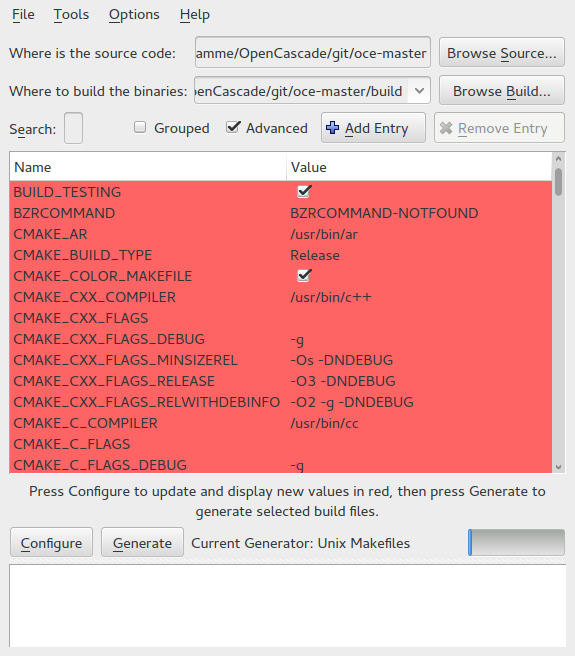
\includegraphics[scale=0.5]{img/CMake_GUI.png}
\caption{CMake graphical interface}
\label{fig:CMake_GUI}
\end{figure}
\subsection{Test OpenCascade}
\begin{figure}
\centering
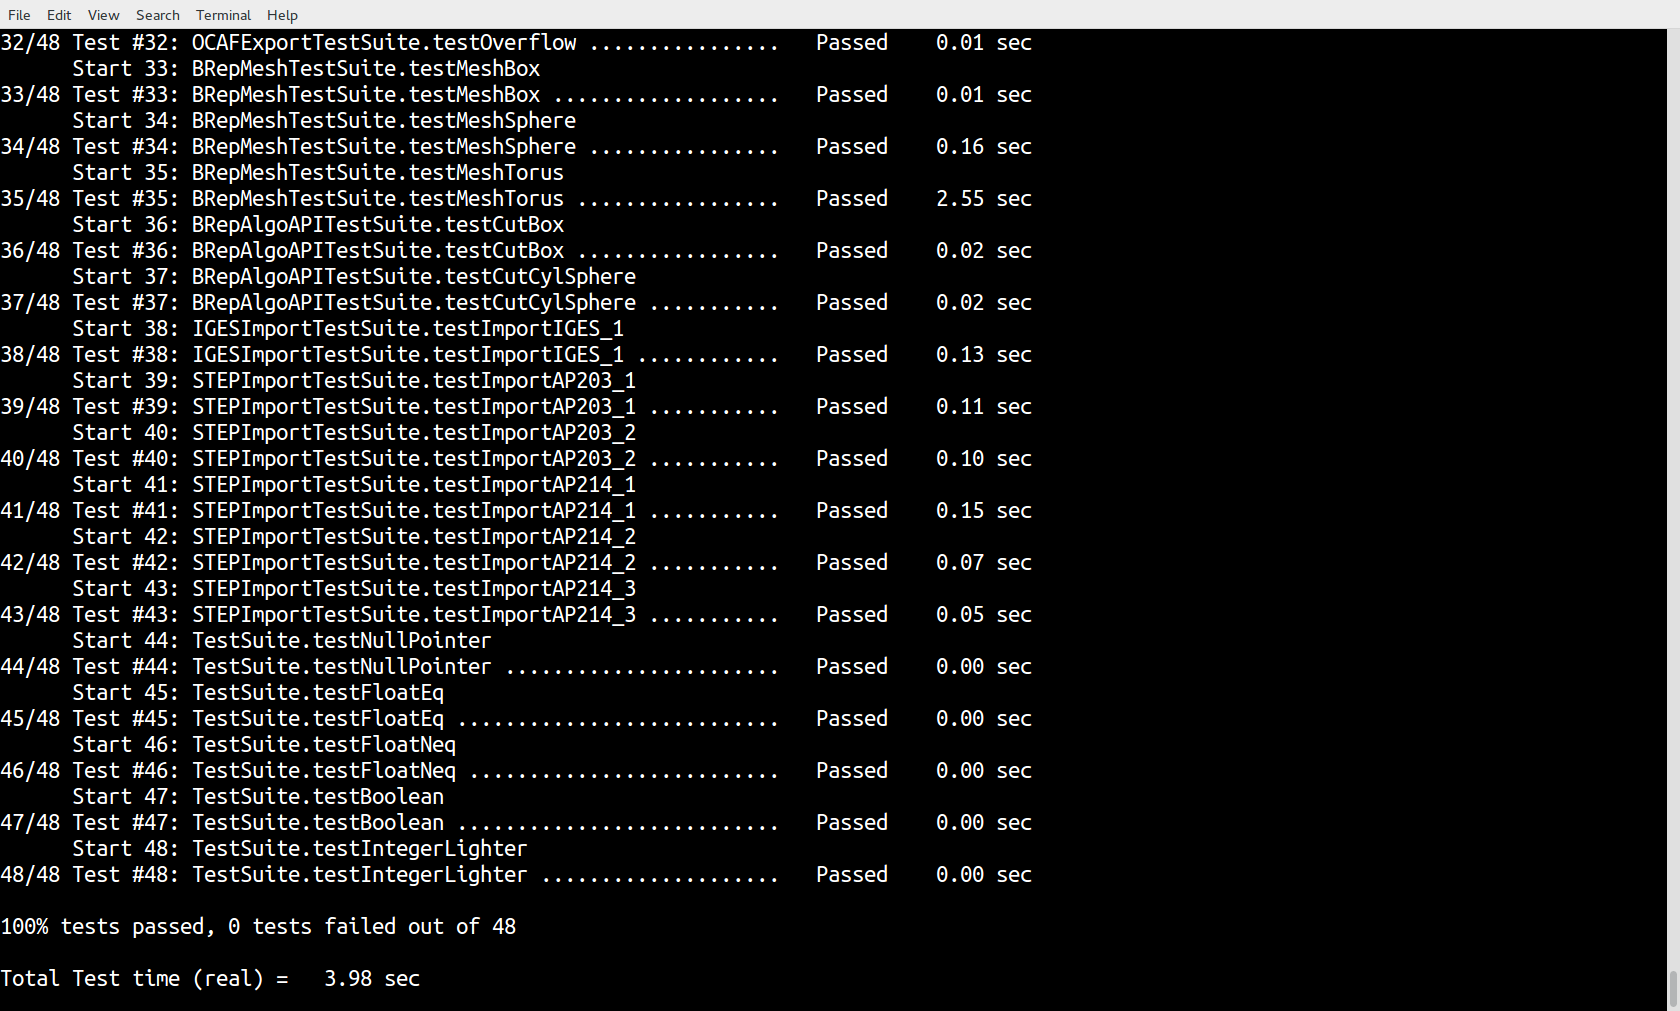
\includegraphics[scale=0.2]{img/OC_Test2.png}
\caption{OpenCascade test}
\label{fig:OC_test}
\end{figure}
In order to test whether the installation of OpenCascade was completed successfully it is possible to run a test provided by OpenCascade. 

For that, run the following command from your terminal:
\begin{itemize}
\item[] \texttt{\textbf{$>$ }make test}
\end{itemize}
All performed tests should be successful (See Pic. \ref{fig:OC_test})

\section{Miscellaneous}
\subsection{Qt \& QtCreator}
\label{Qt}
To install the the newest version of \textbf{Qt}, visit the page \\ \href{http://ftp.fau.de/qtproject/archive/qt/5.4/5.4.2/}{http://ftp.fau.de/qtproject/archive/qt/5.4/5.4.2/} and download the \textit{.run} file suitable for your computer. 
After that, change the rights for the installer file and install \textbf{Qt} by following instructions of the installation manager:
\begin{itemize}
\item[] \texttt{\textbf{$>$ }chmod +x qt-opensource-linux-x64-5.5.0-2.run}
\item[] \texttt{\textbf{$>$ }sudo ./qt-opensource-linux-x64-5.5.0-2.run}
\end{itemize}
\subsection{FreeCAD}
Download and install FreeCAD following the instructions from the official FreeCAD webcite: \\ \href{http://www.freecadweb.org/wiki/?title=Download}{http://www.freecadweb.org/wiki/?title=Download}.

It can also be installed directly from the command line as follows:
\begin{itemize}
\item[] \texttt{\textbf{$>$ }sudo apt-get install freecad}
\end{itemize}

\section{CADO}
\subsection{Prerequisites}
In order to install CADO the following tools should be installed on your computer:
\begin{itemize}
	\item Topy (see Sec. \ref{Topy})
	\item OpenCascade (see Sec. \ref{OpenCascade})
	\item QtCreator (see Sec. \ref{Qt})
	\item FreeCAD
	%\item CPPUNIT (\href{http://cppunit.sourceforge.net/doc/cvs/cppunit_cookbook.html}{http://cppunit.sourceforge.net/doc/cvs/cppunit\_cookbook.html})
	\end{itemize}

After having installed all the prerequisites, CADO is ready to install. To do that, perform the following command from the repository main folder:
\begin{itemize}
\item[] \texttt{\textbf{$>$ }make}
\end{itemize}
After the installation process has completed run the program from the command line:
\begin{itemize}
\item[] \texttt{\textbf{$>$ ./}cado}
\end{itemize}
\end{document}